\documentclass[10pt,handout,english]{beamer}
\usetheme{Berlin}
\usecolortheme{seahorse}
\usepackage{amsmath}

\usepackage{listings}
\definecolor{mymauve}{rgb}{0.58,0,0.82}
\definecolor{mygreen}{rgb}{0,0.6,0}


\usepackage{graphicx} %%For loading image files
\graphicspath{ {images/} } %folder-location for images

\title[] % (optional, only for long titles)
{Python API for Mobile Robot Control}
\subtitle{Progress Presentation-1}
\author[AE-663 Course Project 2016-17] % (optional, for multiple authors)
{Parin Chheda (153076005) \\ Saurav Shandilya (153076004) \\ Group-10 }
\institute [Indian Institute of Technology Bombay]% (optional)
{
  
}
\date[\today] % (optional)
{Prof. Prabhu Ramachandran \\ Prof. Madhu Belur \\ Prof. Kumar Appaiah}
%\subject{Computer Science}

\begin{document} 
	\lstset{language=C,commentstyle=\color{mygreen},showspaces=true,   
		showstringspaces=false, basicstyle=\footnotesize,  
		breakatwhitespace=false,keepspaces=true,            breaklines=true,stepnumber=1,showspaces=false} 
\frame{\titlepage}

\begin{frame}{Objective}
\begin{enumerate}
	\item A Python API to control the different peripherals of the ${\mu}$controller
	\item Provide the user with a option of register level access of the ${\mu}$controller
	\item Allow the user to design an application without learning a new language and thoroughly knowing the architecture of the controller.
\end{enumerate}
\end{frame}

\begin{frame}{System Architecture}

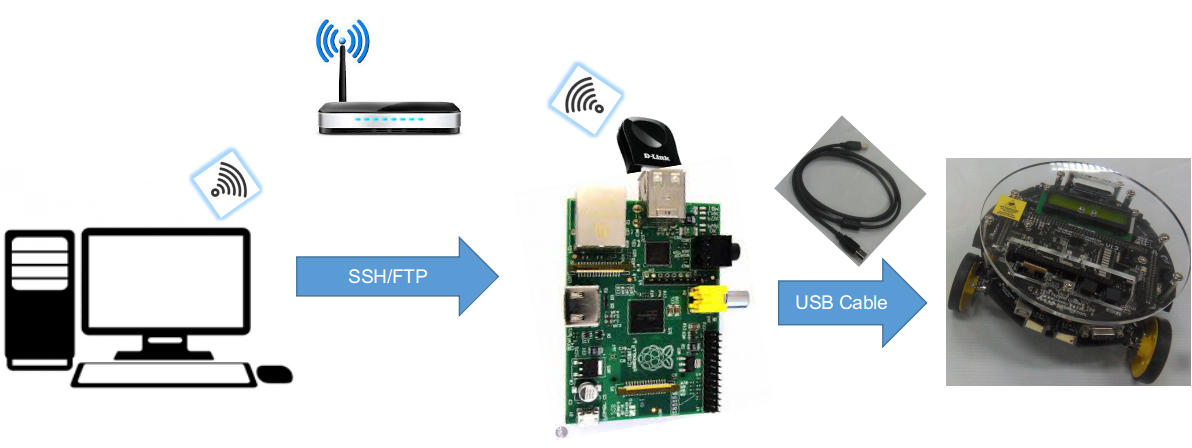
\includegraphics[scale = 0.35]{system_diagram}

\end{frame}

\begin{frame}{Milestone Achieved}
\begin{enumerate}
\item Robot-end firmware - written in embedded C
\item Serial Communication between Raspberry Pi and Robot
\item Function for configuring all IO Ports and Pins of microcontroller
\item Implemented and tested code for Buzzer and BarLED.  
\item Test code for Port and Pin configuration function
\end{enumerate}

\end{frame}

\begin{frame}{User code snippet}
	\lstinputlisting[language=Python]{snippet.py}
\end{frame}

\begin{frame}{Implementation}
Data Packet Format \\[4mm]
\begin{center}
\begin{tabular}{|c|c|c|c|}
\hline  set/rest & Function id & Register id  & Pin value \\ 
\hline  1-bit& 7-bit & 8-bit  & 8-bit  \\ 
\hline 
\end{tabular}
\end{center}

\vspace{3mm}

\textbf{set/reset (1-bit)}: This bit decides whether value a register bit is set high or reset to low \\[1mm]

\textbf{Function id (7-bit)}: These bits select various ${\mu}$controller peripherals Example: IO,ADC,Timers,I2C etc \\[1mm]

\textbf{Register id (8-bit)}: These bits select registers present to access ${\mu}$controller peripherals. Example: DDRA,PORTA, ADCSRA,ADMUX etc \\[1mm]

\textbf{Pin Value (8-bit)}: These bits select value to be written on 8-bit registers


\end{frame}
\begin{frame}{Future Work}
\begin{itemize}
\item Develop and test object-oriented implementation
\item Access following peripherals for ${\mu}$controller
	\begin{itemize}
	\item Timers
	\item ADC
	\item Interrupt
	\item I2C
	\end{itemize}
\item Improve data packet by incorporating checksum, end of packet payload to existing system.
\item Design PyQT GUI for making SFTP connection to Raspberry Pi from PC
\item Provide higher level abstraction for peripheral devices  
\end{itemize}

\end{frame}




\end{document}
